\section{Objetivos}

\subsection{Objetivo Geral}
	O objetivo geral desse projeto é o desenvolvimento de um protótipo totalmente funcional de uma central domiciliar inteligente, baseada no \textit{Raspberry Pi} \cite{magpi} capaz de ser controlada por comandos de voz pelo usuário e capaz de controlar diversos equipamentos elétricos domésticos assim como ser capaz de consultar informações na web.

\begin{figure}[htbp]
	\centering
		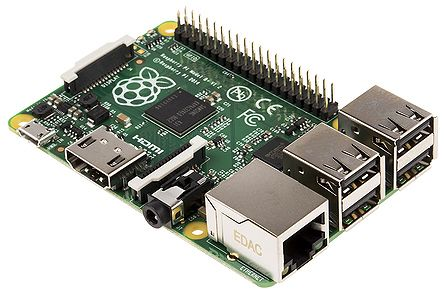
\includegraphics[scale=1.8]{raspberryPi3Board}
	\caption{Raspberry Pi 3 \cite{pi3}}
	\label{fig-raspberrypi3}
\end{figure}

\section{Objetivos Específicos}
  \begin{itemize}
    \item Criar um dispositivo que decodifica sinais sonoros de voz e dispara eventos baseados nessas mensagens.
    \item Criar interfaces e módulos para esse dispositivo afim de garantir integração com outros equipamentos e funcionalidades.
    \item Aplicar os conceitos sobre \textit{IoT}, \textit{UNIX} e programação aprendidos na disciplina de Sistemas Embarcados.
    \item Desenvolver um protótipo de um produto de tecnologia que seja relevante, útil, de forma que não seja algo somente para cumprir os objetivos da disciplina sob qual este projeto se encontra.
  \end{itemize}
